\documentclass[a4paper,11pt]{article}

\usepackage[english]{babel}
\usepackage[utf8]{inputenc}
\usepackage{amsmath}
\usepackage{graphicx}
\usepackage{xcolor}
\usepackage{cite}


%%%%%%%%%%%%%%%%%%%%%%%%%%%%%%%%%%%%%%%%%%%%%%%%%%%
% Students with dyslexia can use an alternative font. To do so, remove the % symbols in front of the three \usepackage commands below.

%\usepackage[T1]{fontenc} 
%\usepackage[bitstream-charter]{mathdesign}
%\usepackage[scaled]{helvet}

%%%%%%%%%%%%%%%%%%%%%%%%%%%%%%%%%%%%%%%%%%%%%%%%%%%

\setlength{\oddsidemargin}{0cm}
\setlength{\evensidemargin}{0cm}
\setlength{\voffset}{-2.5cm}
\setlength{\textwidth}{16cm}
\setlength{\textheight}{25cm}

\title{{\small PHY480 Semester I Project Report}
\\
\vspace{5mm}
Machine Learning and Categorising Objects in the Sky}

\author{160207219}

\date{\today}

\begin{document}
\maketitle

\begin{abstract}
This \LaTeX\ document serves as a template for the PHY480 Autumn Semester report, which is due for submission by the Friday of week 12. The report should have a short abstract, up to about 200 words long, which summarizes the contents of the report.\\

\end{abstract}

\section{Introduction}
\label{sec:introduction}

The report should begin with a brief introduction explaining the context of the work that you are doing for your project. It should explain what your project is about, what you intend to do, and why this is important / useful / interesting. The main body of the report should then follow, broken down into three sections:
\begin{itemize}
\item Literature review.
\item Progress on project.
\item Project plan.
\end{itemize}
The report should finish with a short conclusion.

The total length of the report should be around 5000 words. You can have as many words as you need for your appendices. A quick way to estimate the word count of a \LaTeX\ document is to create a PDF file, select and copy the relevant parts  of the report, and then paste into a word processor that has a word counting facility (e.g. WORD).

The report will be assessed by two academics: your supervisor and another academic. The second academic will normally be someone who works in the same general area as the project topic (e.g. high-energy physics), but will {\em not} be familiar with the details of the project. The marks of the second assessor carry equal weight as those of your supervisor, and so it is important that you explain clearly the context of your project and its aims.

The marks awarded by the two assessors will be averaged, and will count as 25\% of the overall module mark.
The relative weighting of the three components of the report is given in Table~\ref{mark weighting}.

\begin{table}[h]
\caption{Weighting of marks for the PHY480 semester I report}
\begin{center}
\begin{tabular}{|l|c|c|}
\hline
Component & Weighting & Overall module marks \\
\hline
Literature review & 40\% & 10\\
Progress on project &30\%& 7.5\\
Project plan & 10\% & 2.5\\
Writing style & 20\% & 5\\
\hline
\end{tabular}
\end{center}
\label{mark weighting}
\end{table}




\section{Literature Review}
Throughout astronomical history, there was a great need for the classification of objects, be it determining whether the objects are nebulae or stars, or differentiating between different types of active galaxy. However, given the vast amount of data from observations, classifying objects is incredibly costly in terms of human resources. Even from the low resolution images of early photographical plates, one of the most time-consuming parts of data analysis was to identify which objects are important and of those, which ones are the type of object researchers are interested in. Hence, historically, it was difficult to take advantage of the full range of observational data.  

However, with the advent of data processing by computers, it became possible to process ever larger sets of data while maintaining the same level of human resources. This started the process of developing and using various computerised methods to classify data gleaned from observations. This literature review will detail the methods used, from the most primitive methods, to the latest developments in neural networks, of how astronomical objects became classified.
\subsection{Primitive Methods}
From the beginning of astronomical observations, it was determined that some objects are more like others, and hence a classification system was developed. Since the earliest observers had no way of observers to reliably record their observations—they used hand sketches, there was no real need to have mass categorisation of astronomical objects. However, that all changed with the advent of photography. At the turn of the 20th Century, photographic plates to conduct sky surveys and hence build star catalogs became common. This increased the need to devise some kind of classification scheme to make sense of the objects. Such classification schemes can be seen in the Harvard system, or the Hubble Tuning Fork. However, applying such schemes to the objects seen on the sky remained a human endeavour. It would remain so until the 1980s where computing technology advanced to a point in which automated classification was feasible.

In 1988, Adorf \& Meurs applied a classification algorithm to the IRAS catalogue data of extragalactic sources.\cite{adorf_1988_supervised} They compared both supervised and unsupervised methods but did not reach any conclusion on whether either method is better. They made use of AutoClass, a popular machine learning  algorithm at the time. Importantly, they identified two aspects of classification: exploratory and confirmatory. They noted that given a completely unknown set of data, it is much more difficult to make any classification given that one does not know anything 'about' the data. In contrast, confirmatory classification is where one does know the categories that the data must be separated into and therefore the classification is just an exercise in the classification of this data, and hence confirming or denying any hypotheses made about the data. From this, it is clear that to do the former, an unsupervised method is needed to determine the underlying structure of the data, however for the latter, unsupervised or supervised methods will work.

A few years later, a method that could be considered recognisably modern was used to classify the POSS-II sky survey into stars or galaxies.\cite{fayyad_1993_applying} The method starts by doing basic image processing and identifying the sources that need to be classified. The method used is similar to methods used today. Each source then has 18 what they call 'base-level attributes'—what we would call 'feature selection' today—that need to be selected from the source image. These attribute include things like core luminosity and orientation. The attributes for each image are calculated algorithmically and requires no human intervention, however, the attributes themselves are what the researchers determined using our human understanding of how astronomical objects work. While this may make sense prima facie, this is quite a primitive method when compared to modern methods. The reason is this—part of the allure of classification using machine learning is that one can easily stray into the exploration aspect of data science, i.e. using a computer to make sense of data where humans are lacking. While the classification between stars and galaxies may be sufficiently distinct to decide that there is nothing to be gained from allowing a computer to analyse the data sight unseen, that may not be the case when dealing with more subtle classifications, such as those between galaxies types. The algorithm also made use of 'sure-thing stars'. These stars were stars that were hand picked by astronomers within the dataset that were surely stars. This was the beginnings of the creation of a training set. The SkICAT algorithm achieved accuracies of 60-80\% between images, and over 90\% within images. This is a far cry from modern accuracies, but is an achievement considering the time.
\begin{figure}[ht]
\centering
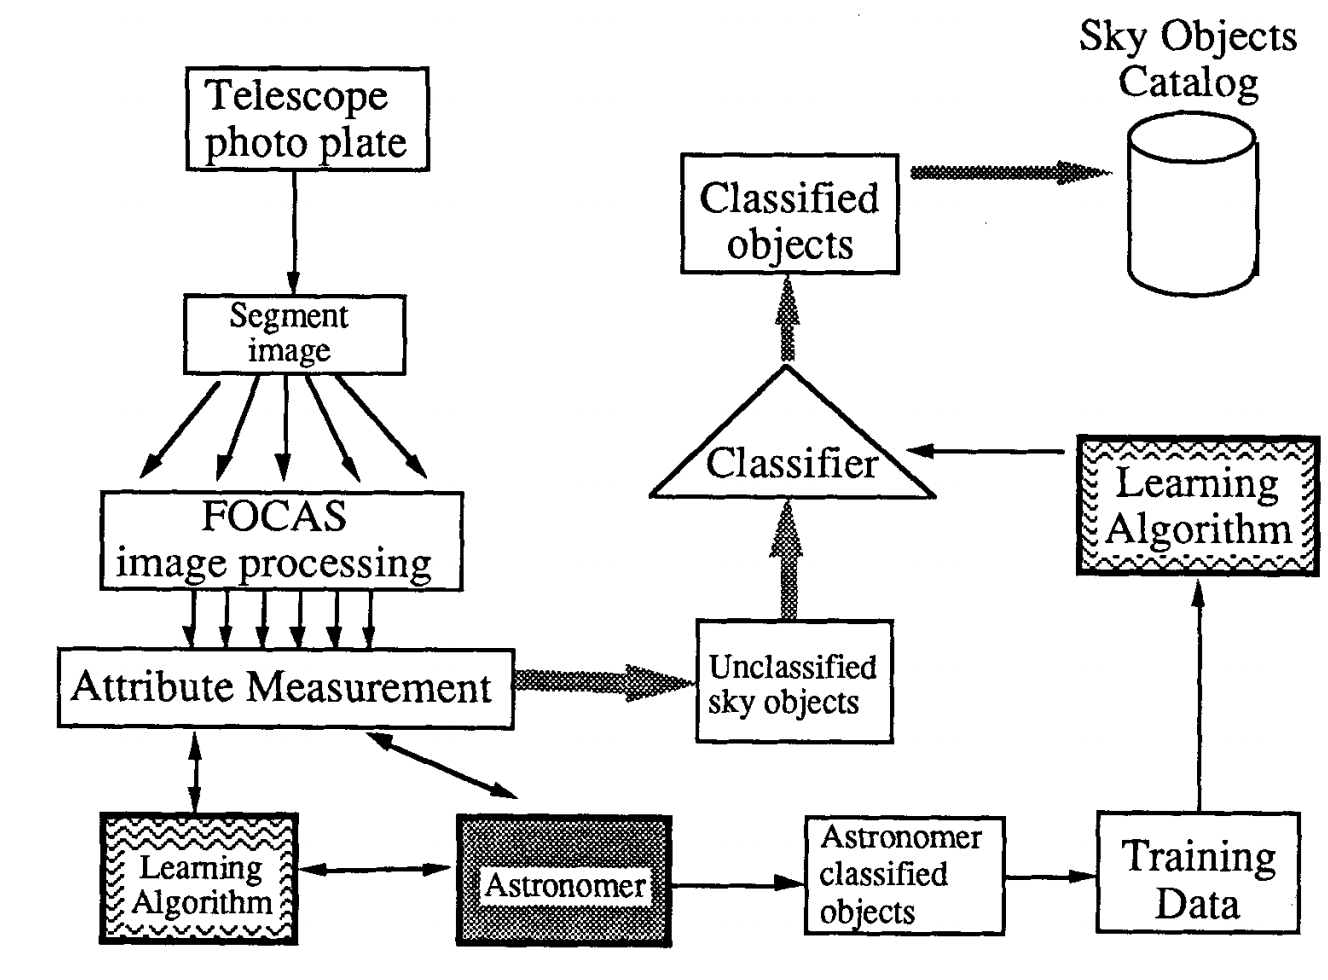
\includegraphics[width=\textwidth]{SkICAT.png}
\caption{\label{fig:SkiCAT}Diagram of the SKICAT algorithm.}
\end{figure}

Further developments in this vein came from Abraham and Merrifield in 2000.\cite{abraham_2000_explorations} They applied largely the same method of manually creating features and then classifying the images according to them. However, instead of classifying galaxies into categories, they placed them in a two dimensional 'Hubble Space' in which one axis is the early/late type classification (cf. Hubble Tuning Fork), and the other is the strength of the bar. Then, they found that the distribution was not uniform and there were groups of galaxies such as ellipticals, spirals and barred spirals. They then classified these galaxies according to these groups. What they  performed was dimension reduction followed by a primitive method of clustering. Clustering is a machine learning tool used to identify the 'clusters' in data. Clustering is an unsupervised method because it does not require humans to indicate what the clusters should be. However, in this case it is difficult to determine whether the resulting groups are a result of choosing the two parameters. 
\begin{figure}[ht]
\centering
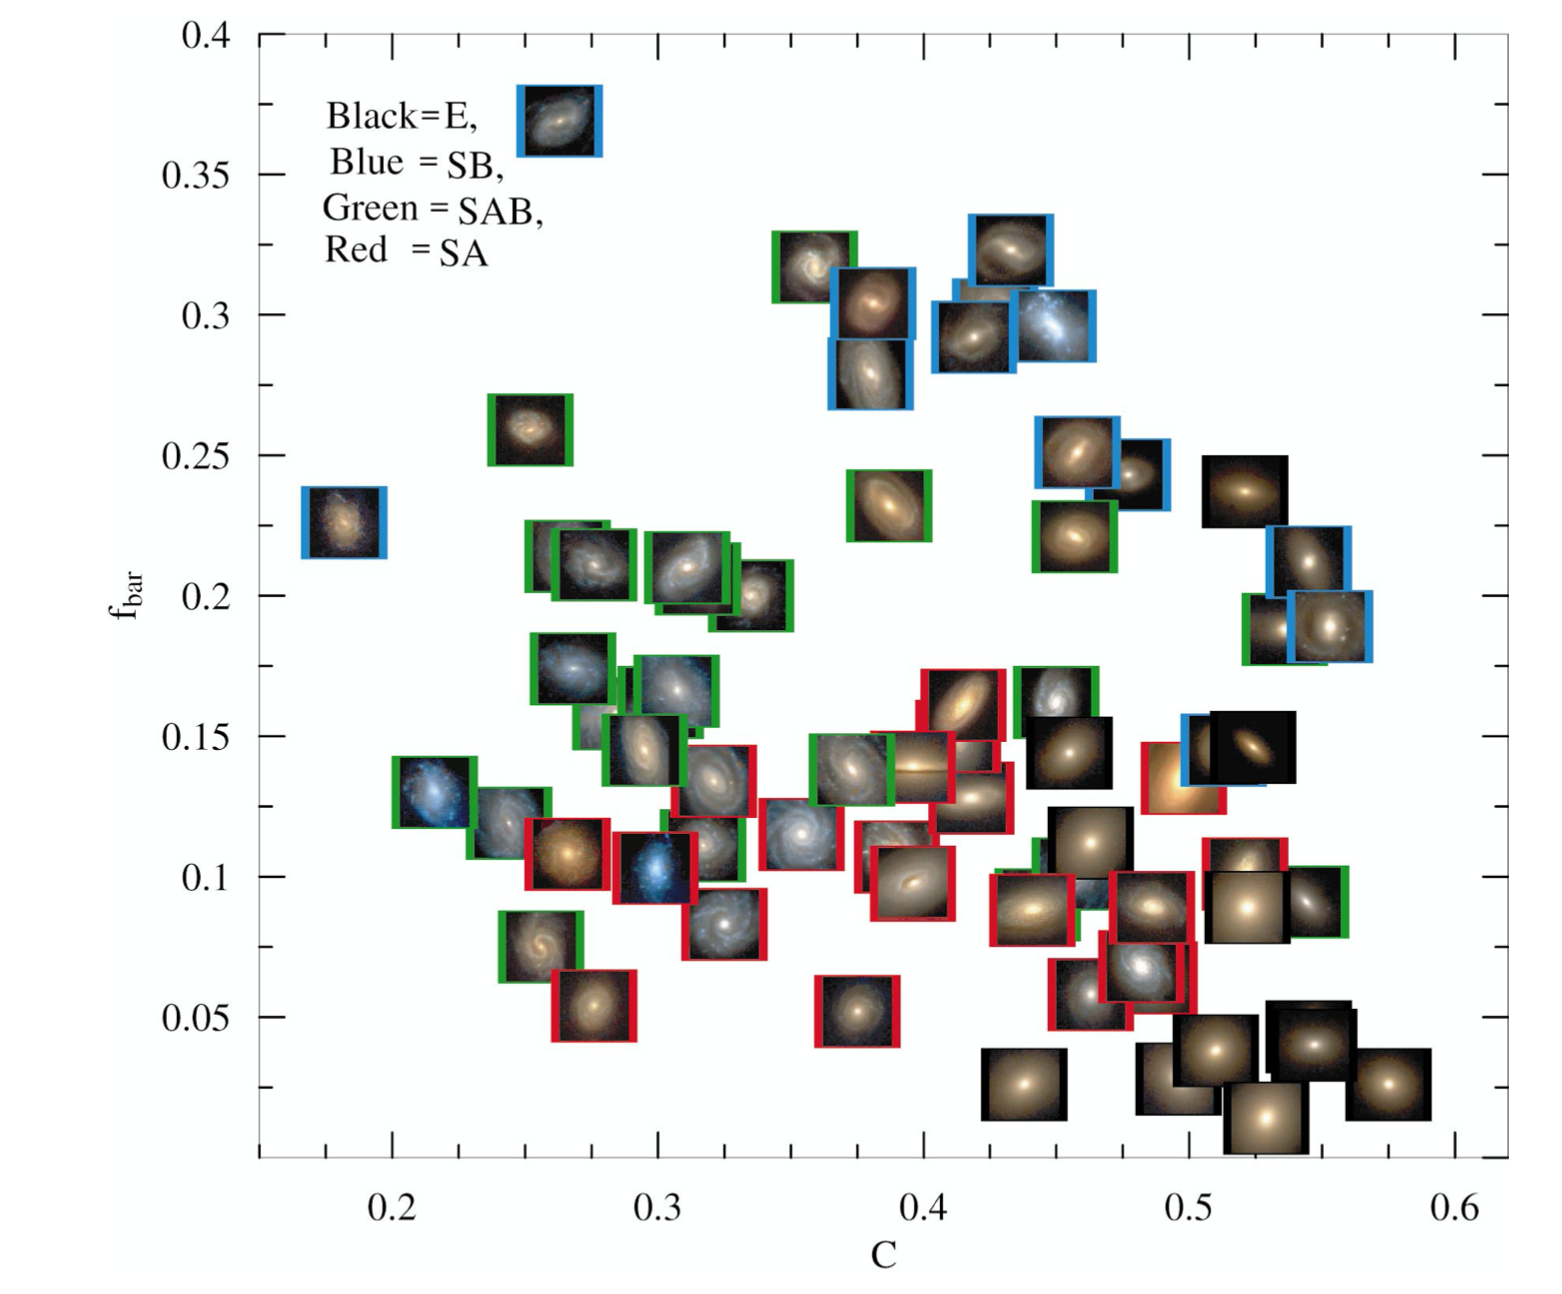
\includegraphics[width=\textwidth]{Abraham.png}
\caption{\label{fig:Galaxies}The distribution of galaxy images in their sample within Hubble Space}
\end{figure}

\subsection{Support Vector Machines and Principal Component Analysis}
\subsubsection{Support Vector Machines}
In order to understand support vector machines (SVM), one must first understand the earlier logistic regression algorithm. Logistic regression operates on a sample by separating it on two classes. It makes use of the logistic function:
\begin{equation}
h_{\theta}(X)=\frac{1}{1+e^{\theta^{T}X}}
\end{equation}
where $h_\theta X$ is a 'generalised linear parameter'. The key effect of this is that any such 'dividing' line(or hyperplane when there are more dimensions) that successfully splits the parameter space into two according to the training data is a 'good' split. However logistic regression gives no indication on how good a particular fit is. That is the motivation for developing SVM.

Without getting into the specifics of the algorithm, when training either logistic regression or SVM, a cost function must be found. The cost function in the logistic regression is smooth while in SVM is a hinge loss. This enables it to measure the 'goodness of fit'. SVM tries to maximise the margins between the hyperplane and the closest data point to either side of it. This is useful in many cases because SVM gives the 'best' classifier in some description of the word. 
\begin{figure}[ht]
\centering
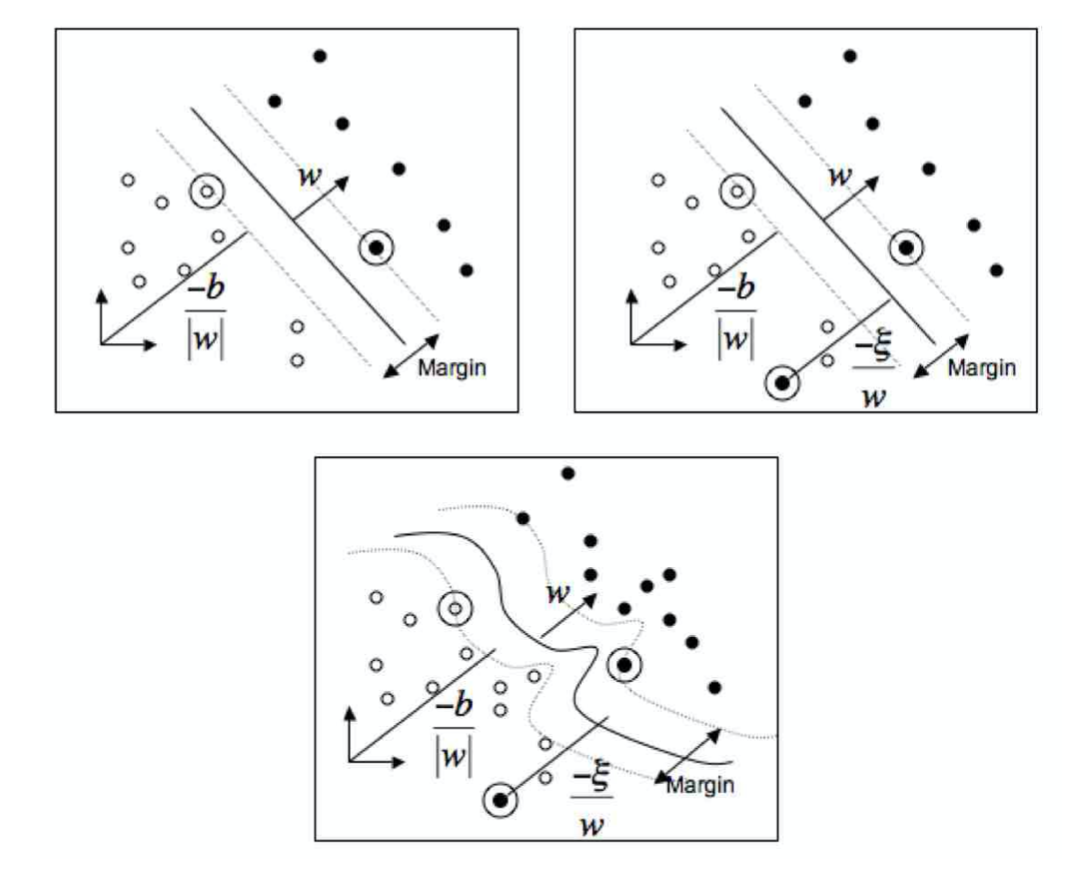
\includegraphics[width=\textwidth]{SVM.png}
\caption{\label{fig:SVM}A figure showing how SVM works. The upper left shows SVM with linearly separable data. The upper right shows SVM with non linearly separable data. The bottom shows kernel SVM with non linearly separable data.}
\end{figure}
\subsubsection{Principal Component Analysis}
The motivation of principal component analysis (PCA) is to reduce the dimensionality of data while preserving as much information as possible. This is useful because reducing the dimension of data makes it much less computationally expensive to manipulate it. The underlying theory of PCA is beyond the scope of this literature review, but in broad brushes, PCA makes use of some matrix manipulations to find the eigenvalues/eigenvectors of the marix of data. This is then further manipulated to give a set of components (so-called principal components), which are sorted in accordance to how much of the information they retain from the original data. The first component will have most of the information and the second will have less, and so on. If one chooses to truncate the components at some value, one can still be certain that they will have 'most' of the information retained. This tool is greatly useful because it is not very computationally expensive, with computational complexity of $O(\min(p^3,n^3))$ \cite{johnstone_2009_on}, where n is the number of data points and p is the number of features. However, this method loses meaning on the specific components resulting from the algorithm because each principal component is some linear combination of all the original components.
\subsubsection{SVM and PCA as applied to astronomical classification}
SVM and PCA started to be applied to astronomical classification in the early 2000s. Calleja and Fuentes were one of the earlier applications of PCA to astronomical classification.\cite{delacalleja_2004_automated} They used PCA and a variety of classification algorithms to classify galaxies from the SDSS. 8, 13, and 25 principal components were used to perform their classification because they represent 75\%, 80\%, 85\% of the information from the data. Note how the marginal benefits of including many more principal components are diminishing as a result of PCA. They made use of a number of classifiers, with a Random Forest classifier being the best. They found that when classifying into 3 classes the accuracy is 91.64\%; 5 class: 54.72\%; 7 class: 48,62\%. This indicates that there are probably 3 'true' classes in the data. However this is not known until further clustering analysis is done on them.

Conselice \cite{conselice_2006_the} found that, using over 20000 galaxies in the sample, the principal components after performing a PCA analysis on the sample largely matched what was predicted using human methods. He found that the 3 main components are scale, star forming regions, and galaxy interactions/merger. From this, he developed a 3 axis classification of galaxies. However, he notes that real galaxies are much more 'messy', and this is one of the key points from this paper—real life objects do not fit cleanly into categories assigned. Therefore, it is quite possible that objects are simply unclassifiable or are otherwise not suitable for the classification system assigned, hence, the blind pursuit of 100\% accuracy is ill founded and inadvisable.

Huertas-Company et al \cite{huertascompany_2007_a} wrote two papers on using SVM to classify galaxies. They reduced the data down to 12 parameters and performed SVM on them. The classification was performed to separate them into two groups—early and late types. They found that with the WIRCam sample, the accuracy only reached 60\% while for the better SDSS sample, the accuracy reached 80\%. However, this is to be expected as the 12 parameters for the galaxies do not seem to be linearly separable.

In their subsequent paper \cite{huertascompany_2010_revisiting}, the group used a pre-built SVM classifier to classify the data. They attempted to further classify the two classes and therefore split each of the classes into two; ultimately forming 4 classes: E, S0, Sab, Scd. From their paper, it was apparent that the pre-built classifier was performing a 'kernel-SVM', or using SVM with a 'kernel trick'. This trick transforms the originally linearly inseparable data to a higher dimension using the eponymous kernel. This allows the data to be linearly separable in some higher dimension. In fact, the mathematics guarantee that there are an infinite number of kernels which can be used, and at least one of them is linearly separable (gaussian kernels map the data to infinite dimensional space, which makes the data linearly separable). 
\begin{figure}[ht]
\centering
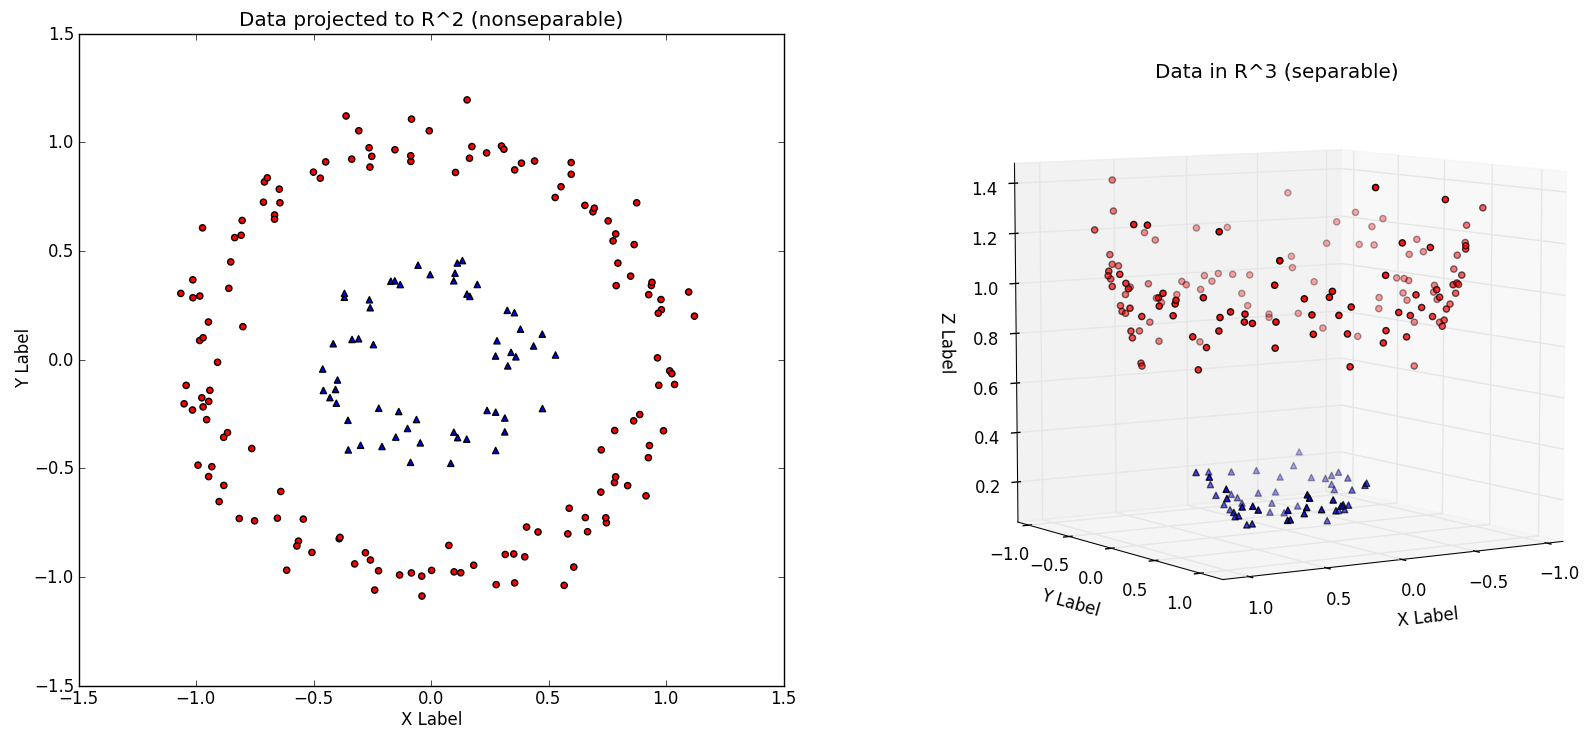
\includegraphics[width=\textwidth]{kernelSVM.png}
\caption{\label{fig:kernelSVM}When data is mapped to a higher dimension, it might make it linearly separable when it previously was not. (Towards Data Science)}
\end{figure}

The group, using this method achieved greater success in their classification, with a scatter of 12\%, it may be assumed that their accuracy was 88\%. They also mentioned that 0.4\% of objects were considered unclassifiable.  

This shows the power of a relatively old method—SVM, which can be updated to compete with more modern methods, and this may be a a way forward in binary classifiers.

\subsection{Neural Networks}
Neural networks are so termed because they are similar to the way neurons in the human brain work. There are several types of neurons in neural networks, but broadly speaking they perform simple calculations, pass the information forwards or backwards, and retain the information for a period of time. When these neurons are combined, they form neural networks (NNs). 
\begin{figure}[ht]
\centering
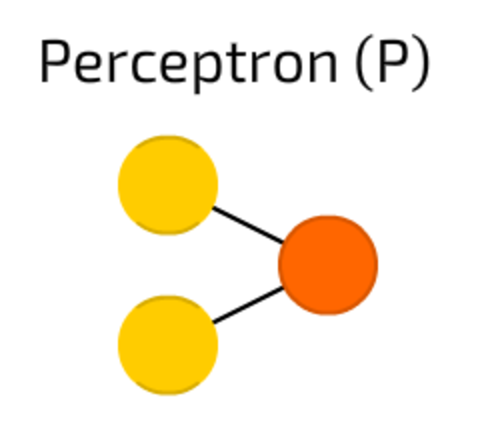
\includegraphics[width=0.25\textwidth]{Perceptron.png}
\caption{\label{fig:Perceptron}A Perceptron is the simplest neuron. It takes in numbers and performs a sum. They may be simple classifiers. (Towards Data Science)}
\end{figure}
\subsubsection{Artificial Neural Networks}
Artificial neutral networks (ANNs) are not a type of neural network per se, rather, they stand in contrast with the convolutional neural networks that will be discussed later. ANNs are so termed because they make use of a neural architecture that is pre-determined. All ANNs require features to be selected beforehand, by a human, or by an algorithm like PCA. The simplest of these ANNs is the feedforward neural network (FNN). The concept of an FNN has existed since the 50s, but they are not very useful since they only have one layer.
\begin{figure}[ht]
\centering
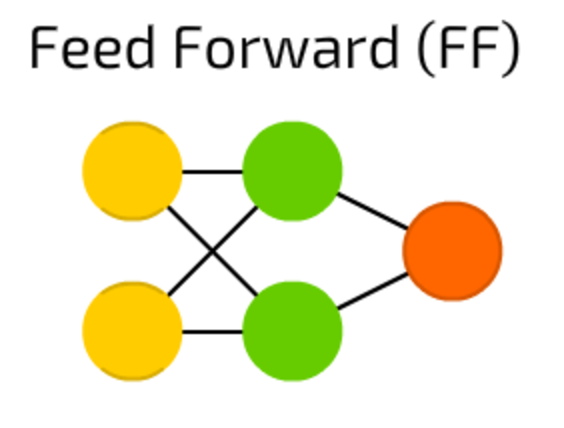
\includegraphics[width=0.25\textwidth]{FNN.png}
\caption{\label{fig:FNN}A FNN comprises of a fully connected network that only passes information forward. (Towards Data Science)}
\end{figure}

The FNN concept can be easily extended by increasing the number of layers between the input and the output layer. A FNN that has more than one layer is called a Deep FNN (DFNN). 

\begin{figure}[ht]
\centering
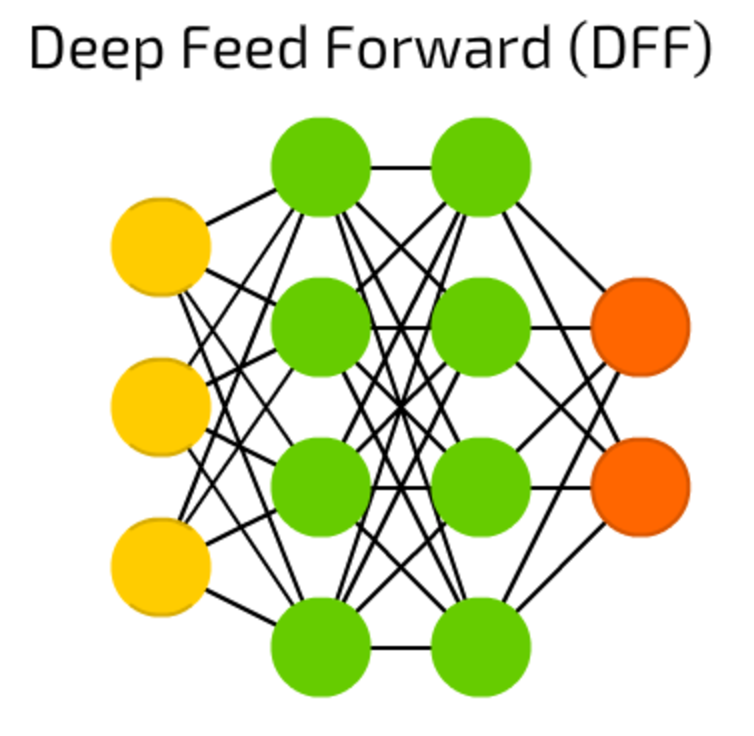
\includegraphics[width=0.25\textwidth]{DFF.png}
\caption{\label{fig:FNN}A DFNN is simply a FNN with more layers. It retains the characteristics of being fully connected and information only passed forwards.(Towards Data Science)}
\end{figure}

The DFNN arose in the 90s, where the methods to train them finally existed—previously, because of the nature of error propagation, errors would accumulate through the network and eventually cause the network to fail entirely. Now, it is used in lieu of the simple FNN and produces superior results. Further, in the area of classification, having only one layer only allows the network to classify linearly separable data, while networks with more than one layer does not have this limitation.

Another type of artificial neural network that is relevant today is the recurrent neural network (RNN). A RNN is in essence a FNN with the nodes replaced by recurrent nodes. A recurrent node is simply a node which feeds itself as an input to itself after a time-delay. 
\begin{figure}[ht]
\centering
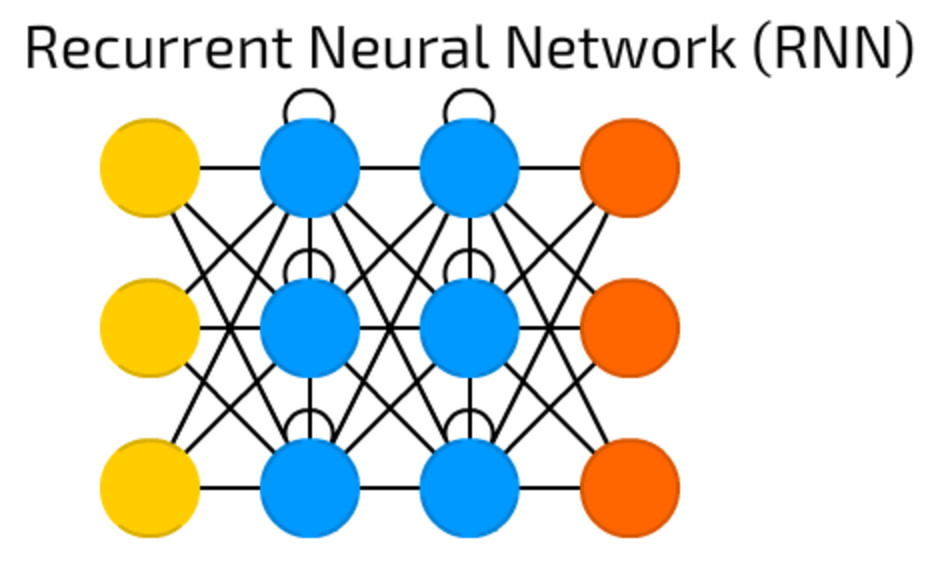
\includegraphics[width=0.25\textwidth]{RNN.png}
\caption{\label{fig:RNN}An RNN is very similar to an FNN, in fact it has the same structure except it changes the nodes from only feeding forward to being recurrent.(Towards Data Science)}
\end{figure}

RNNs are used today in applications where context is sensitive, like natural language processing. However, given the nature of astronomical images, this does not seem like a viable or useful path.

Because convolutional neural networks are inherently more suited to image processing, work on the field of applying ANN to astronomical classifications is very limited. The only work on the field seems to be to classify spectral data—because spectral data is not imagery in nature.\cite{hampton_2017_using} However, even that seems to be very lacking.

\subsubsection{Convolutional Neural Networks}
Convolutional neural networks(CNNs) are structurally very similar to FNNs, the difference here is that the activation functions of those nodes are not simple activation functions, but rather convolutional and pool activation functions. 
\begin{figure}[ht]
\centering
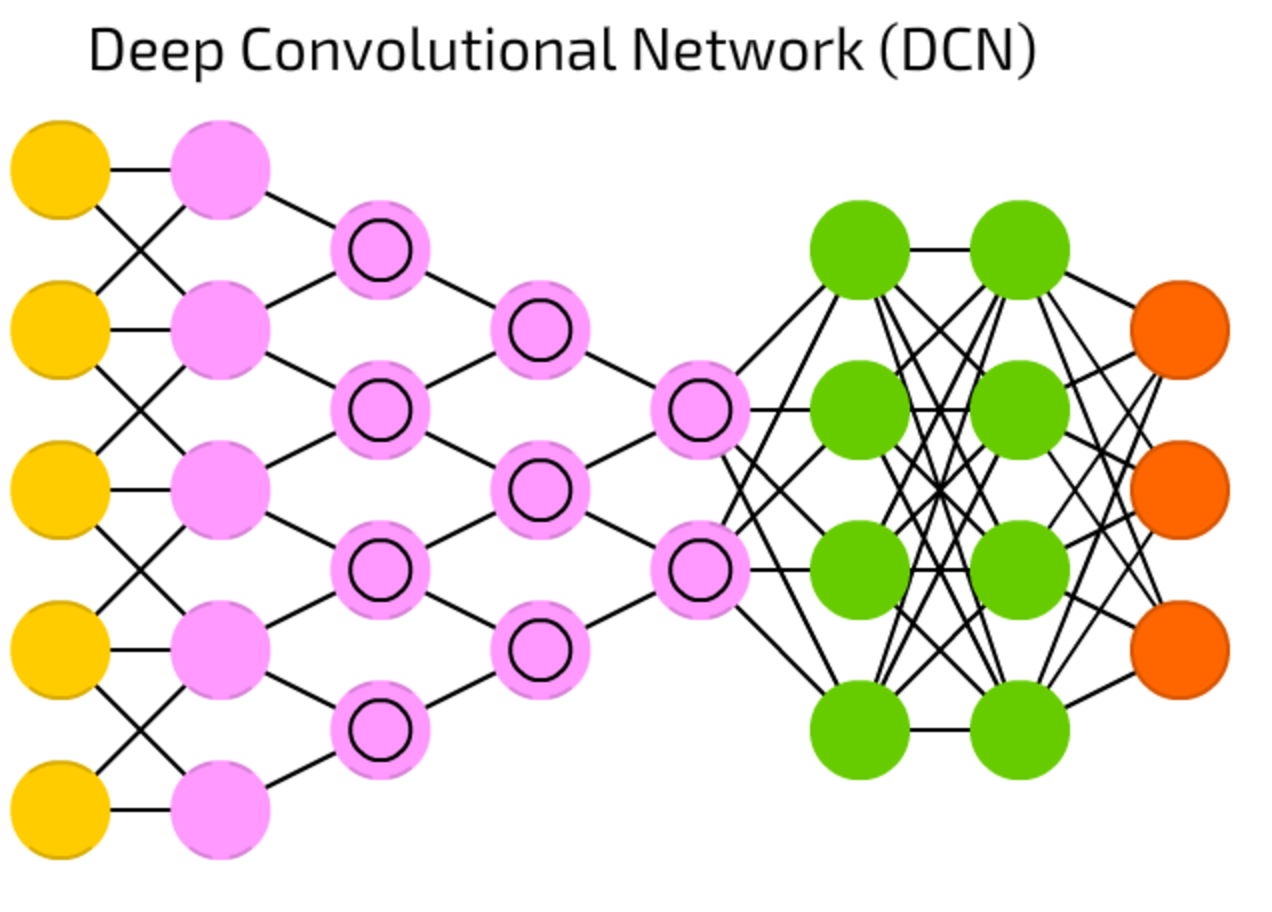
\includegraphics[width=0.25\textwidth]{CNN.png}
\caption{\label{fig:CNN}A CNN uses convolution and pooling layers instead of feedfoward nodes. Note that FNNs are frequently used at the end of CNNs for further data processing.(Towards Data Science)}
\end{figure}

However, in practice this is very different. Since convolution functions act on images rather than specially selected features, they avoid requiring features to be selected from the images.

CNNs have been extensively used in galaxy classification since the late 2010s. There are various approaches using a differing combination of convolutional hidden layers and pooling layers as well as varying levels of hardware capability. Kim \& Brunner \cite{kim_2016_stargalaxy} made use of 5 band images to classify galaxies. They used a structure with 8 convolutional layers, 3 pooling layers and 2 fully connected layers. They achieved an accuracy of 95-98\% depending on which accuracy metric is used. However, in their discussion they mentioned that there was a lack of training data to train with, and this seemed to be a problem which is shared with others working with CNNs. \cite{khalifanoureldeenm_2017_deep} \cite{aniyan_2017_classifying} The reason for this seems unclear to me as there is not a dearth of astronomical data, in fact there is a wealth of such data, why they are not able to acquire such data is quite curious to me.

From the literature, it is also quite clear that there are not too many astronomers truly using CNNs for classification, rather, it seems the wealth of literature is of computer scientists using astronomy data as a proof of concept for their CNNs. And these all garner results of over 95\% with very little data. However, the benefit of computer scientists doing the research is that their code is freely avaliable on repositories such as github.

The path of CNNs seem very promising if one has sufficient data, and data is not lacking in this project. 

\subsection{Galaxy Zoo}
When training neural networks, copious amounts of training data is needed. One method of acquiring such training data is through sky surveys, but another is through citizen science projects like Galaxy Zoo. \cite{lintott_2008_galaxy}

The Galaxy Zoo project was a massive project which harnessed the power of average people to classify images from sky surveys. The accuracy of those classification collectively are on par with the best neural networks. Further, the classified data is freely available online, and therefore is easily used as training data. This approach has already been tried by some groups. Banerji has used Galaxy Zoo data to train a neural network and achieved 90\% accuracy. \cite{banerji_2010_galaxy} However unfortunately he does not specify what kind of neural network he is using and so it is impossible to verify whether the accuracy is due to deficiencies in his neural network or in the Galaxy Zoo data. 

\subsection{Exotic Methods}
There are more exotic methods attempted in the literature to classify galaxies. One of which is Hocking et al \cite{hocking_2017_an} , who used a 'neural gas' in an unsupervised classification algorithm. They attempted to replicate findings by the Galaxy Zoo Project in the CANDELS field. They discovered that the classifications somewhat matched what a human classifier would identify (early/late types). Such unsupervised methods had also been attempted earlier by Schutter \& Shamir, \cite{banerji_2010_galaxy} albeit to somewhat less success. 

Another method which is equally exotic is Abd Elaziz et al. They used an artificial bee colony to classify galaxies. \cite{abdelaziz_2018_galaxies} The results were comparable to using SVM. 

However, the point of these exotic methods is not necessarily to be immediately applicable, but they may drive new developments in the field generally that may one day be somehow applied to astronomical classifications.

\subsection{Summary}
After delving into the literature, it seems that the methods most immediately applicable to the current project is PCA/SVM and CNNs. Using these methods, it is possible to classify stars and galaxies, and between types of galaxies. CNN in particular is still in its infancy, there are still very much room for the field to expand and develop. 

\newpage
\label{sec:theory}

You should write a literature review of the background to the research that you are conducting. You should aim to explain why your topic is of interest to the scientific community, and then summarize what work has already been done on the subject. You will need to cite the key papers that underpin your research. See \cite{Einstein} for an example. You should use standard scientific style, providing the following information: 
\begin{itemize}
\item author(s);
\item title of paper;
\item journal name, volume number, pages (or article ID number), year.
\end{itemize}
If you cite books \cite{good book} or longer review articles, you should give the specific section of the book to which you are referring. 
If you are uncertain about how to do the citations, then you can refer to the physics referencing tutorials provided by the library.
The references can either be numbered (as in this report template), following AIP style~\cite{AIP style}, or they can follow the Harvard (name, date) system~\cite{Harvard style}, which is the  style common in astronomy journals. 
You might also find it helpful to use BibTeX (http://www.bibtex.org/) in the LaTeX template and EndNote (https://www.sheffield.ac.uk/cics/endnote) for Word documents.


There is no limit to the number of references, and the appropriate number depends on the nature of the project.  You should therefore discuss the papers that you intend to cite with your supervisor.  As a general guide, a typical literature review would cite between 10 and 20 references. In some cases, however, it might be appropriate to focus in depth on a relatively small number, while in others it may be necessary to have more than 20 references. You should be selective about what you cite, and demonstrate that you have read the cited material. 
 Note that, even if there are only one or two papers that are directly relevant to your specific task, there will be a general body of literature that puts the research topic in its context.
 
The use of figures can greatly improve the presentation of your literature review. If you do include figures, you first need to generate an image file (JPEG, PNG or PDF), and then use the {\tt includegraphics} command to include it in your document. Make sure that the axis labels are easily readable be ageing assessors with poor eyesight. Use the {\tt figure} environment and the {\tt caption} command to add a number and a caption to your figure. See the code for Figure \ref{fig:eclipse} for an example. Make sure that the original source of the figure is dutifully acknowledged. There is no limit to the number of figures you can include.

An electronic copy of your report must be submitted with your printed copies. The electronic copy will be analysed with the Turnitin anti-plagiarism tool. You should therefore make sure that you comply stringently with the University's plagiarism guidelines. See \cite{plagiarism}. Note that minor changes to the original wording do not constitute a defence against accusations of plagiarism: you have to genuinely use your own words.

If you are uncertain about any aspects of referencing and plagiarism, then please look up the on-line tutorials provided by the library \cite{Referencing}. You should work through, at least, the tutorial on understanding plagiarism and one of the referencing tutorials listed under Physics \& Astronomy. 



\begin{figure}
\centering
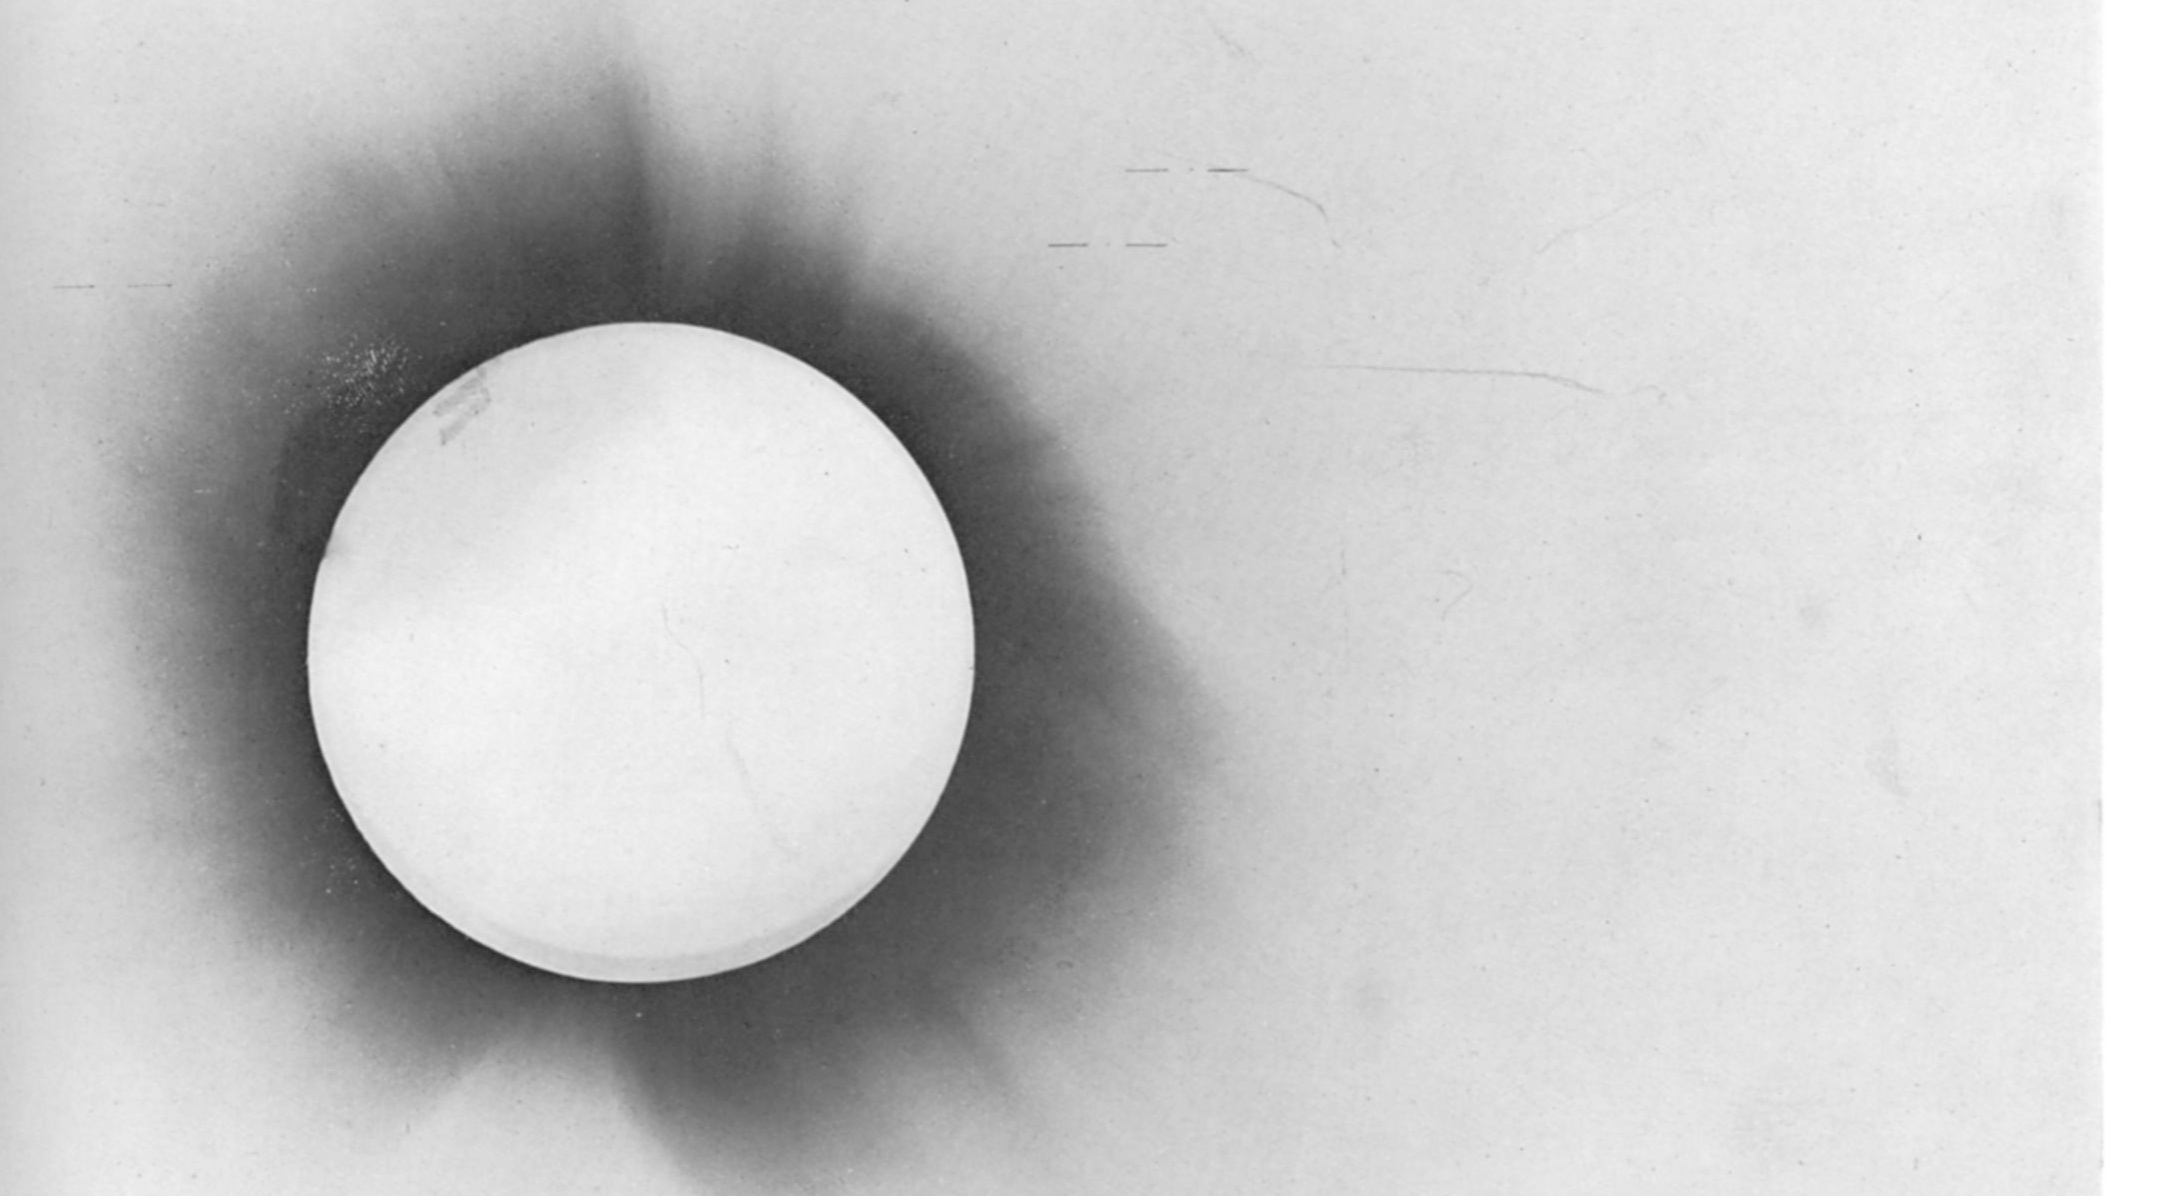
\includegraphics[width=\textwidth]{Dyson.jpeg}
\caption{\label{fig:eclipse}Solar eclipse of 1919, which was studied to prove the bending of light by gravity. From \cite{Dyson}.}
\end{figure}





\section{Progress on Project}
You should provide a description of the preparatory work and development of background skills that you have undertaken during the first semester of your project. The contents of this section will be dependent on the nature of your project. Early results may be given, but are not a required element, as your ability to generate results during Semester~I will depend on the nature of the work. \textbf{Risk assessments are obligatory} for all experimental projects, and should be included as appendices, with appropriate discussion in the main text.

Your report should reflect the actual work you have done so far, providing evidence that you have put in the time expected of students during the 1st semester of PHY480. You should describe, concisely, any techniques or skills you have developed in the early stages of your project,
using appropriate scientific language. You should avoid the use of jargon, but if you do use jargon or acronyms, they should be defined before use. All equation should be numbered, following standard scientific style, as in eqn~\ref{E=mc2}.
\begin{equation}
\label{E=mc2}
E = m\,c^2 \, .
\end{equation}
If you wish, you may add appendices to present your preliminary results in more detail or to list any computer code you have written. In some projects, it might be appropriate to summarize the key findings in a table.



\section{Project Plan}
You should give a plan for the work to be carried out next semester, in as much detail as you think appropriate. Each project plan element should consist of a brief description of the task, a realistic estimate of the time it will take to complete this task, and an achievement milestone that indicates task completion. The number of tasks should be realistic, and the project should be broken down into appropriately sized components. It might be appropriate to present the project plan as a Gantt chart: see~\cite{gannt}.

Note that your project plan has to be reproduced verbatim in the semester II report, and that the semester II report should include a discussion of how well you kept to your plan. Research is, by definition, unpredictable, and so there is no shame in departing from your plan, provided that you had a good reason to do so. However, you should be able to defend your change of course, and this is what you are asked to do in your report.  

\section{Relationship to previous projects}
If you have already completed a project in the group where you are working, you should include a $\sim 1$-page statement indicating how the PHY480 project differs from previous work. This is especially important if you are building on previous work done, for example, during a summer project. You must state clearly the new work that you have done during this semester. This statement should be attached as an appendix.

\section{Submitting the report}

You should submit \textbf{three} printed copies of your report and an electronic version by Friday of week 12 of the Autumn Semester. Your printed reports should be mounted in the plastic binders that can be collected from F10. You should use the \LaTeX\ or WORD templates that are provided on MOLE to prepare your report. Do not change the font size or margins in the templates, and the report should be in single-column format. An alternative \LaTeX\  font is available for students with dyslexia. Please see the preamble to the \LaTeX\  template file.





\newpage

\bibliographystyle{Alpha}
\bibliography{Semester 1 report}



\newpage 
\begin{appendix}

\section{(Where appropriate) Relationship to previous projects}
If you have already completed a project in the group where you are working, you should include a $\sim 1$-page statement indicating how the PHY480 project differs from previous work. This is especially important if you are building on previous work done, for example, during a summer project. You must state clearly the new work that you have done during this semester.
\newpage

\section{Risk assessments}
You should attach as many risk assessment as are needed. These are obligatory for experimental projects.

\end{appendix}


\end{document}
              
    
